% Chapter 1

\chapter{Introduction} % Main chapter title

\label{Chapter1} % For referencing the chapter elsewhere, use \ref{Chapter1} 

%----------------------------------------------------------------------------------------

\section{User friendly Data analysis: gAn Web}

GAn is a program that aims to analyse data related to the AEgIS experiment at the CERN, gAn Web is the web interface of gAn, and it is the main topic of this document.
 
This program receive in input (from another software system) several terabytes of files in ".root" format, and some input parameters inserted by the user; 
It does an analysis and it gives in output some summarized scientifically interesting information, understandable by humans.   
A file ".root" is a file produced by a variegated group of sensors in a complex machine that accelerates particles and lets them crash together. This sensors produce data continuously (8 hours per day), and a software system validates and saves these data in file with .root extension. 

The input parameters are:
\begin{enumerate}

% 1
\item "Run Number", that identifies in which part of the data the user is interested. 
The time in this experiment is divided in "runs" (a run lasts about some hundred seconds), so the user, by the run parameter can tell to gAn in which time slice he is interested. For example: run 55614 means that the user is interested in the information related to the 22th of November 2016, taken in the time slice between 15:45 and 15:47. 
The enumeration of the runs is incremental: so the run 55199 identifies the time slice immediately after the time slices identified by 55198. The progress of the run numbers is always going on, so new run numbers are continuously added. 
In this document every time we say "last run number" we don't mean the absolute last run numbers, but the run number that is going on right in this moment. This concept is important because usually in most cases the users use gAn Web on the last existing run number (so on the run number that is going on right at that moment) or the immediately previous run number.  
This system to identify time slices seems to be strange at the beginning but is a standard for all the applications in the AEgIS experiment and it allows a very efficient and precise communication.

How can the user have more information about the runs? 
On another server exists a RunLog (sometimes also called LogBook). The RunLog is a document organized by date on which at each run a group of person write the run number, some informations (about settings), some observation (at maximum 2 rows, usually one.. so usually brief observations [but if in the run something particular happens, in that rare case the observations can become very long] ). 
Is this document an input or an output for gAn Web? it depends:
If the user uses gAn Web on the last existing run (or the run immediately before) probably the output of gAn Web is one of the (many) input of the RunLog.  
If the user is interested in a phenomenon happened some days ago, probably he searches on the RunLog at the page related the date of the phenomenon, he choose one or more runs related to this phenomenon (he recognize them by the observations), he works with gAn using these runs, and probably he notes parts of the output of gAn Web as observations on the RunLog, that in this situation is both input and output. Some runs are absolutely not related with gAn Web, so in some cases the RunLog is neither an input nor an output.  

% 2
\item "Type of analysis", that identifies what the program must do with the data and what it must show as output to the user.
A "type" is a way in which the program extracts information from the raw data. each type can extract different information using different parts of data and elaborating them in different ways. For example: a type of analysis named "Tmeas" can extract information about the temperatures of some elemental particles analysing how quickly they move subjected to a force. 

\end{enumerate}


The .root files can be analysed using a framework named ROOT Framework, that consists in a lot of libraries specialized in high-energy physics analysis, and an interpreter able to understand a C++ script.
Actually, gAn is the sum of the Root Framework plus a lot of C++ scripts.
The goal of gAn is reduce the big amount of raw data received in input in a little amount of scientifically interesting and easily understandable data in output. To do this it has to filter data, understand which of them are scientifically interesting, chose the parts that are related to the run selected by the user (by the run parameter), elaborate and compare them, and make advanced statistical analysis on them.  
gAn can be called using a common linux terminal, using a command with parameters. 

The output of gAn consists of a single text file with computed, (quite) organized data, and a folder of images in png format.
This structure (root files in input, data analysis using Root, images, organized and selected data in output) is very common in the CERN's experiments. 
The output of gAn is quite understandable by an experienced physicist, but it is disorganized, complex for an untrained user, and the terminal interface can be surely improved using some more user friendly technologies.

GAn Web is a web application, that aims to create a user friendly web interface, based on the most important human-machine interaction principles, between the users and gAn.
A web interface can improve the system in two ways:

\begin{enumerate}

% 1
\item gAn is a stand-alone program based on Root, installable on the user's machine; the user has to install the correct version of Root to avoid compatibility problems (Root is still not perfectly version independent: different versions can lead to different behaviours). Furthermore, this kind of program is continuously changing, the performed analysis is continuously improved (in the first 2 weeks from the debut of the program there are already several different kinds of analysis, because often at the changing of the needs the programmers creates new generations of analysis), so the installed version of gAn is not final and unchangeable, and the user musts often update it. Instead, a centralized version installed on a server, with services accessible from a normal browser by the user can avoid (at least reduce) this kind of problems and be more usable.    
 

% 2
\item a Linux terminal interface is practical for expert users, but a web based interface can be more attractive for new users, and, if well done, can be easier to use. It is important to notice that the users are physicists, not necessarily specialized in computer science, so, create a friendly and easily learnable interface can avoid them problems and time wasting.   


\end{enumerate}


The goal of gAn Web is to allow users to do analysis through a more friendly web interface, without install nothing on their machine. In the following image there is a schema that shows how this program is organized.

\begin{figure}[H]
\centering
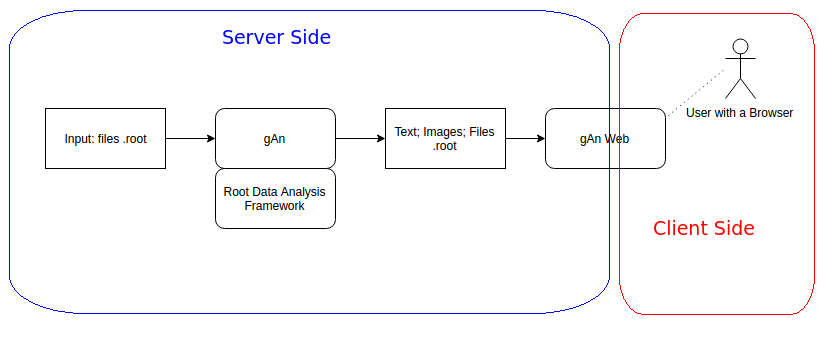
\includegraphics[scale=0.5]{GeneralGAnSchema.png} 
\caption{gAn - gAn Web simple scheme}
\end{figure}



